\section{Process Discovery}
\subsection{Alpha Miner}

\begin{exercise}{1}
Given the following event log:
\[L_1 = [\langle a,b,c,d \rangle^3, \langle a,c,b,d \rangle^2, \langle a,e,d \rangle^1]\]
build the process model using the Alpha Miner algorithm.
\end{exercise}
\paragraph{Solution}
\begin{enumerate}
    \item First, we need to compute the footprint matrix.
    We build a matrix, with all activities in the log as both rows and columns.
    Each cell \((x,y)\) will contain the relation between activity \(x\) and activity \(y\):
    \begin{itemize}
        \item \(\rightarrow\) if \(y\) directly follows \(x\) in some trace, but not vice versa;
        \item \(||\) if both \(x\) and \(y\) directly follow each other in some traces.
        \item \(\#\) if there is no direct relation between \(x\) and \(y\).
    \end{itemize}
    The table is symmetric along the diagonal, so we only need to compute one half of it:
    \begin{table}[H]
    \centering
    \begin{tabular}{c|ccccc}
        & A & B & C & D & E \\
        \hline
        A & $\#$ & $\rightarrow$ & $\rightarrow$ & $\#$ & $\rightarrow$ \\
        B &  & $\#$ & $||$ & $\rightarrow$ & $\#$ \\
        C &  &  & $\#$ & $\rightarrow$ & $\#$ \\
        D &  &  &  & $\#$ & $\leftarrow$ \\
        E &  &  &  &  & $\#$ \\
    \end{tabular}
    \caption{Footprint Matrix for the Event Log \(L_1\)}
\end{table}
    \item Next, we identify the sets of all transitions $T_L$, the set of start activities $T_I$ and the set of end activities $T_O$:
    \begin{itemize}
        \item $T_L = \{a,b,c,d,e\}$, always corresponds to the rows/columns of the footprint matrix;
        \item $T_I = \{a\}$, since every trace starts with activity \(a\);
        \item $T_O = \{d\}$, since every trace ends with activity \(d\).
    \end{itemize}
    \item Then, we identify the pairs of sets of transitions that satisfy the Alpha Miner conditions.
    To find the first pairs, we look for causality relations in the footprint matrix:
    \[\{
        (\{a\}, \{b\}),\\
        (\{a\}, \{c\}),\\
        (\{a\}, \{e\}),\\
        (\{b\}, \{d\}),\\
        (\{c\}, \{d\}),\\
        (\{e\}, \{d\})
    \}\]
    \item We can then group these pairs into maximal sets. For example, since we have both \((\{a\}, \{b\})\) and \((\{a\}, \{e\})\),
    and there is no causality relation between \(b\) and \(e\), we can group them into \((\{a\}, \{b,e\})\).
    Continuing this process, we obtain:
    \[\{
        (\{a\}, \{b,e\}),\\
        (\{a\}, \{c,e\}),\\
        (\{b,e\}, \{d\}),\\
        (\{c,e\}, \{d\})
    \}\]
    We can then remove the non-maximal pairs used to compose them, resulting in:
    \[\{
        (\{a\}, \{b,e\}),\\
        (\{a\}, \{c,e\}),\\
        (\{b,e\}, \{d\}),\\
        (\{c,e\}, \{d\})
    \}\]
    \item Finally, we can construct the Workflow net:
    \begin{itemize}
        \item We create a place \(p_i\) as the input place, and connect it to all activities in \(T_I\);
        \item We create a place \(p_o\) as the output place, and connect all activities in \(T_O\) to it;
        \item We create one place for each of the identified maximum sets and connect them to the activities, 
        according to the causality relations:
    \end{itemize}
    The resulting Petri net is the following:
    \begin{figure}[H]
        \centering
        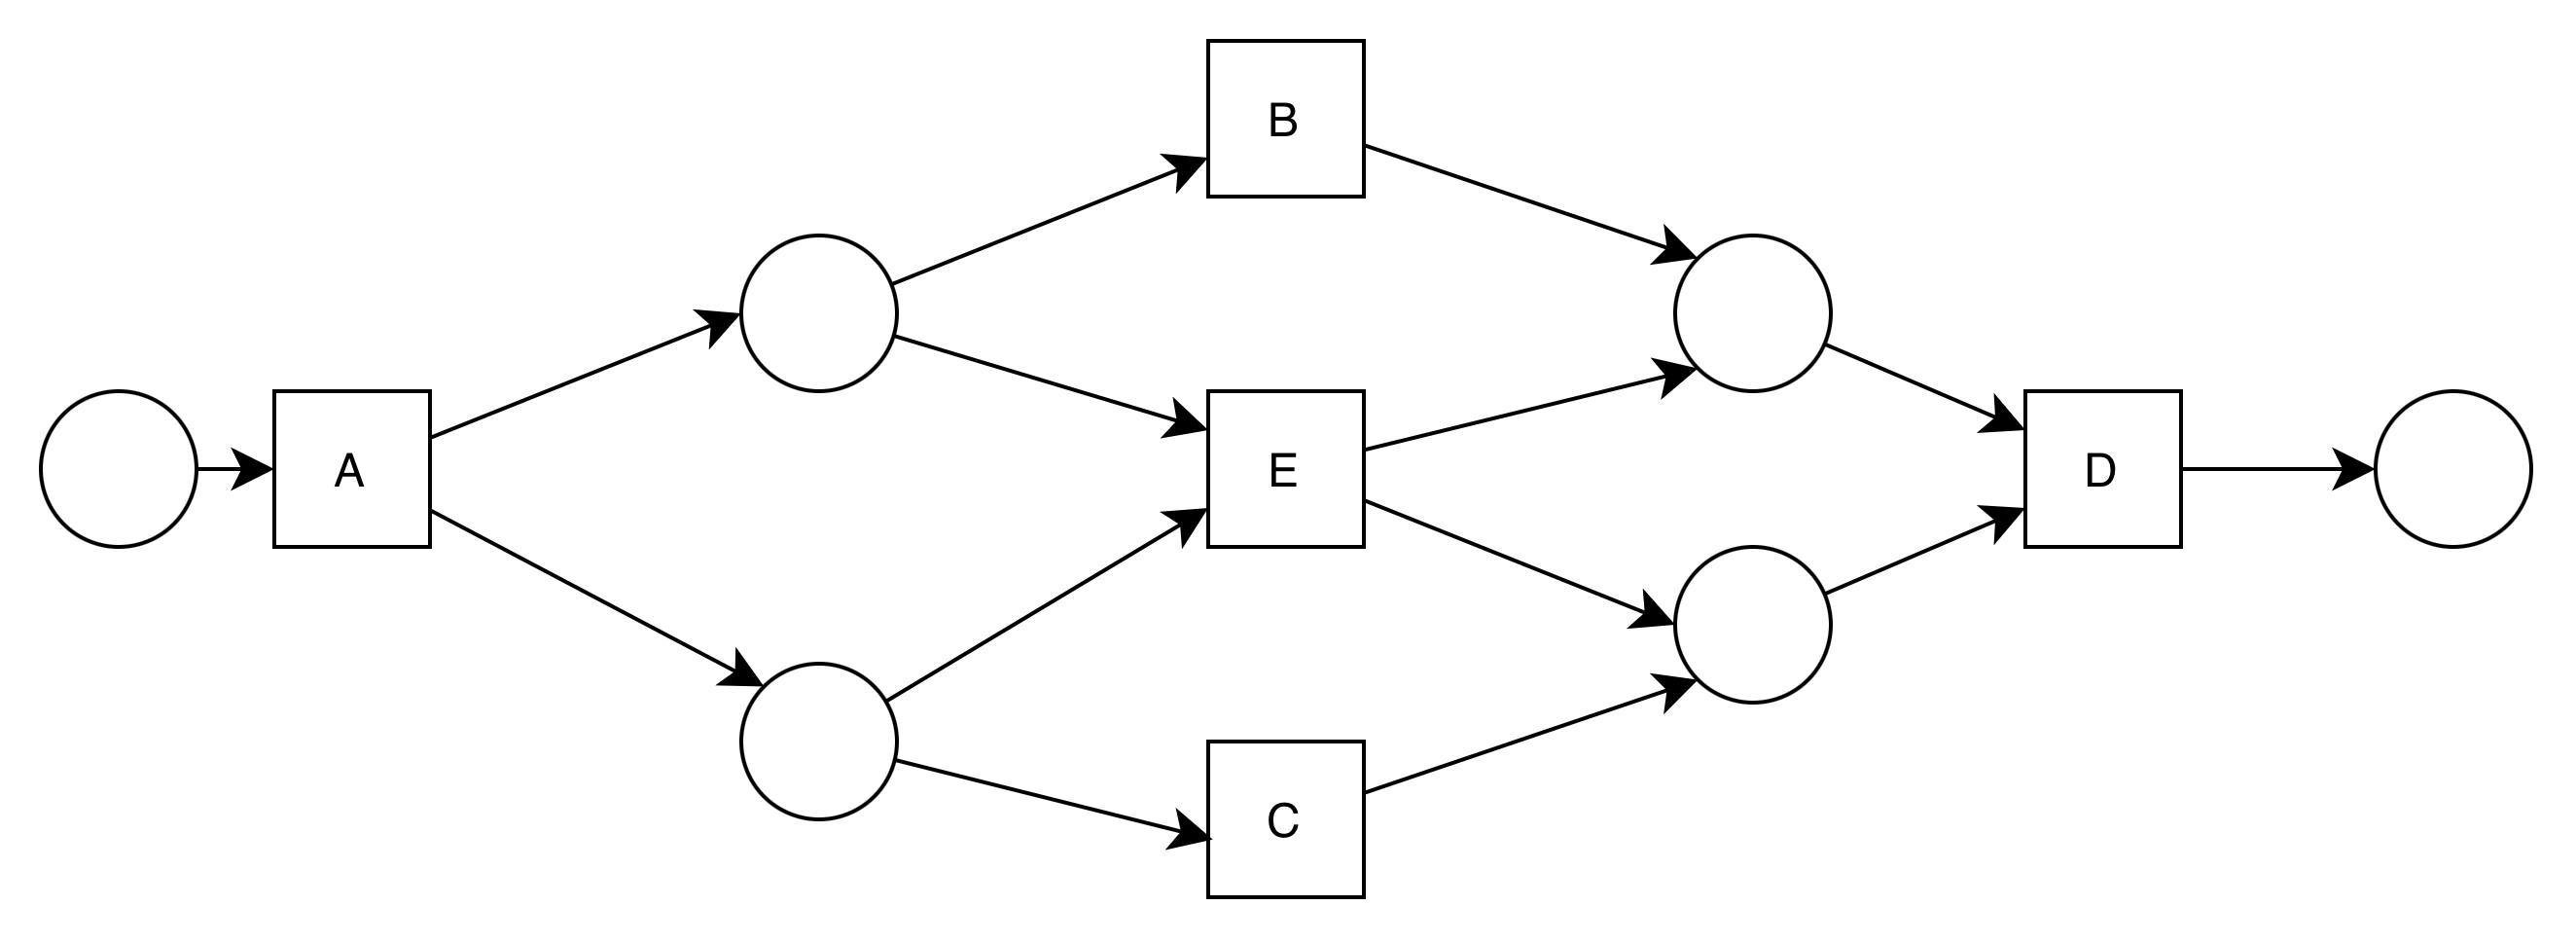
\includegraphics[width=0.7\textwidth]{../images/exercises/proc_discovery/alpha_miner-1.png}
        \caption{Petri Net Discovered using the Alpha Miner}
    \end{figure}
\end{enumerate}

\begin{exercise}{2}
Given the following event log:
\[L = [ \langle a,b,c,d,e,f,b,d,c,e,g \rangle, \langle a,b,d,c,e,g \rangle^2,\] 
\[\langle a,b,c,d,e,f,b,c,d,e,f,b,d,c,e,g \rangle]\]
Use the Alpha Miner algorithm to discover a Petri net from the event log.
\end{exercise}
\paragraph{Solution:}
\begin{enumerate}
    \item First, we need to compute the footprint matrix:
    \begin{table}[H]
    \centering
    \begin{tabular}{c|ccccccc}
        & A & B & C & D & E & F & G \\
        \hline
        A & $\#$ & $\rightarrow$ & $\#$ & $\#$ & $\#$ & $\#$ & $\#$ \\
        B &  & $\#$ & $\rightarrow$ & $\rightarrow$ & $\#$ & $\leftarrow$ & $\#$ \\
        C &  &  & $\#$ & $||$ & $\rightarrow$ & $\#$ & $\#$ \\
        D &  &  &  & $\#$ & $\rightarrow$ & $\#$ & $\#$ \\
        E &  &  &  &  & $\#$ & $\rightarrow$ & $\rightarrow$ \\
        F &  &  &  &  &  & $\#$ & $\#$ \\
        G &  &  &  &  &  &  & $\#$ \\
    \end{tabular}
    \caption{Footprint Matrix for the Event Log \(L\)}
\end{table}
    \item Next, we identify the sets of all transitions $T_L$, the set of start activities $T_I$ and the set of end activities $T_O$:
    \begin{itemize}
        \item $T_L = \{a,b,c,d,e,f,g\}$
        \item $T_I = \{a\}$
        \item $T_O = \{g\}$
    \end{itemize}
    \item Then, we identify the pairs of sets of transitions that satisfy the Alpha Miner conditions.
    \[
    \{
        (\{a\}, \{b\}),\\
        (\{b\}, \{c\}),\\
        (\{b\}, \{d\}),\\
        (\{f\}, \{b\}),\\
        (\{c\}, \{e\}),\\
        (\{d\}, \{e\}),\\
        (\{e\}, \{f\}),\\
        (\{e\}, \{g\})
    \}
    \]
    \item We can then group these pairs into maximal sets and remove the non-maximal ones used to compose them.
    \[
    \{
        (\{a,f\}, \{b\}),\\
        (\{e\}, \{f,g\}), \\
        (\{b\}, \{c\}),\\
        (\{b\}, \{d\}),\\
        (\{c\}, \{e\}),\\
        (\{d\}, \{e\}),\\
    \}
    \]
    \item Finally, we can construct the Workflow net, using one place for each of the identified pairs, and connecting them according to the causality relations:
    \begin{figure}[H]
        \centering
        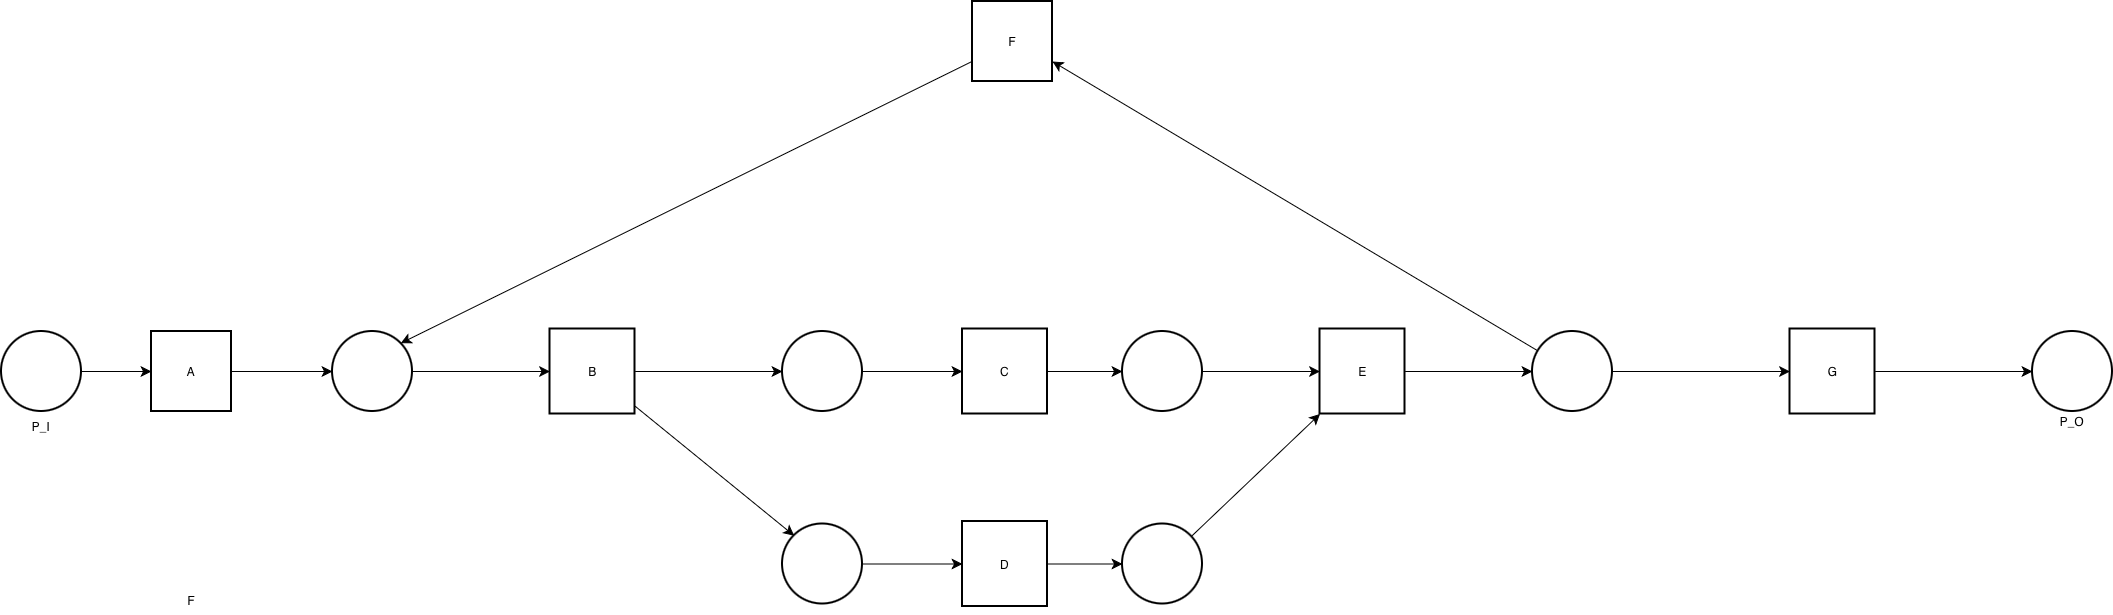
\includegraphics[width=0.7\textwidth]{../images/exercises/proc_discovery/alpha_miner.png}
        \caption{Petri Net Discovered using the Alpha Miner}
    \end{figure}
\end{enumerate}

\begin{exercise}{3}
Given the following event log:
\[L_4 = [\langle a,c,d \rangle^{45}, \langle b,c,d \rangle^{42}, \langle a,c,e \rangle^{38}, \langle b,c,e \rangle^{22}]\]
build the process model using the Alpha Miner algorithm.
\end{exercise}
\paragraph{Solution:}
\begin{enumerate}
    \item First, we need to compute the footprint matrix:
    \begin{table}[H]
        \centering
        \begin{tabular}{c|ccccc}
            & A & B & C & D & E \\
            \hline
            A & $\#$ & $\#$ & $\rightarrow$ & $\#$ & $\#$ \\
            B &  & $\#$ & $\rightarrow$ & $\#$ & $\#$ \\
            C &  &  & $\#$ & $\rightarrow$ & $\rightarrow$ \\
            D &  &  &  & $\#$ & $\#$ \\
            E &  &  &  &  & $\#$ \\
        \end{tabular}
        \caption{Footprint Matrix for the Event Log \(L\)}
    \end{table}
    \item Identify the sets:
    \[T_L = \{a,b,c,d,e\}\]
    \[T_I = \{a,b\}\]
    \[T_O = \{e,d\}\]
    \item Identify the maximal pairs:
    \[\{
        (\{a\}, \{c\}),\\
        (\{b\}, \{c\}),\\
        (\{c\}, \{d\}),\\
        (\{c\}, \{e\})
    \}\]
    \[\{
        (\{a,b\}, \{c\}),\\
        (\{c\}, \{d,e\})
    \}
    \]
    \item Finally, we can construct the Workflow net:
    \begin{figure}[H]
        \centering
        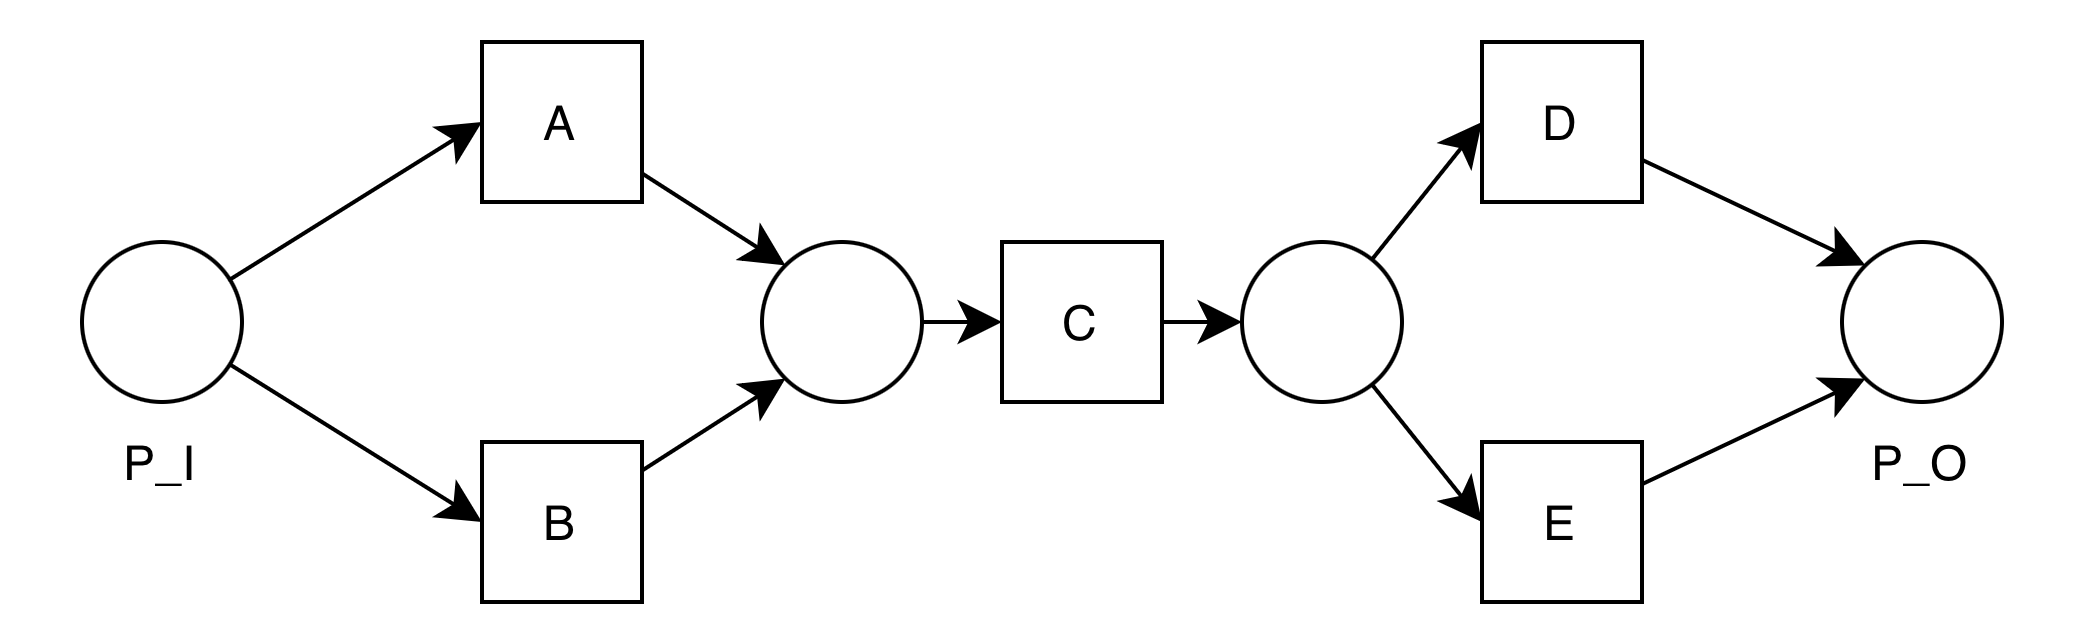
\includegraphics[width=0.5\textwidth]{../images/exercises/proc_discovery/alpha_miner-3.png}
        \caption{Petri Net Discovered using the Alpha Miner}
    \end{figure}
\end{enumerate}

\begin{exercise}{4}
Consider the following event log:
\[L = [\langle a,b,d \rangle^{100}, \langle a,c,b,d \rangle^{80}, \langle a,b,c,d \rangle^{2}, \langle a,c,d \rangle^{40}, \langle a,d \rangle^{1}]\]
Use the Alpha Miner algorithm to discover a Petri net from the event log.
\end{exercise}
\begin{itemize}
    \item First, we compute the footprint matrix:
    \begin{table}[H]
        \centering
        \begin{tabular}{c|cccc}
            & A & B & C & D \\
            \hline
            A & $\#$ & $\rightarrow$ & $\rightarrow$ & $\rightarrow$ \\
            B &  & $\#$ & $||$ & $\rightarrow$ \\
            C &  &  & $\#$ & $\rightarrow$ \\
            D &  &  &  & $\#$ \\
        \end{tabular}
        \caption{Footprint Matrix for the Event Log \(L\)}
    \end{table}
    \item Next, we identify the sets:
    \[T_L = \{a,b,c,d\}\]
    \[T_I = \{a\}\]
    \[T_O = \{d\}\]
    \item We can then identify the maximal pairs:
    \[ 
        \{
        (\{a\}, \{b\}),\\
        (\{a\}, \{c\}),\\
        (\{a\}, \{d\}),\\
        (\{b\}, \{d\}),\\
        (\{c\}, \{d\})
        \}
    \]
    No bigger sets can be formed.
    \item Finally, we can construct the Workflow net:
    \begin{figure}[H]
        \centering
        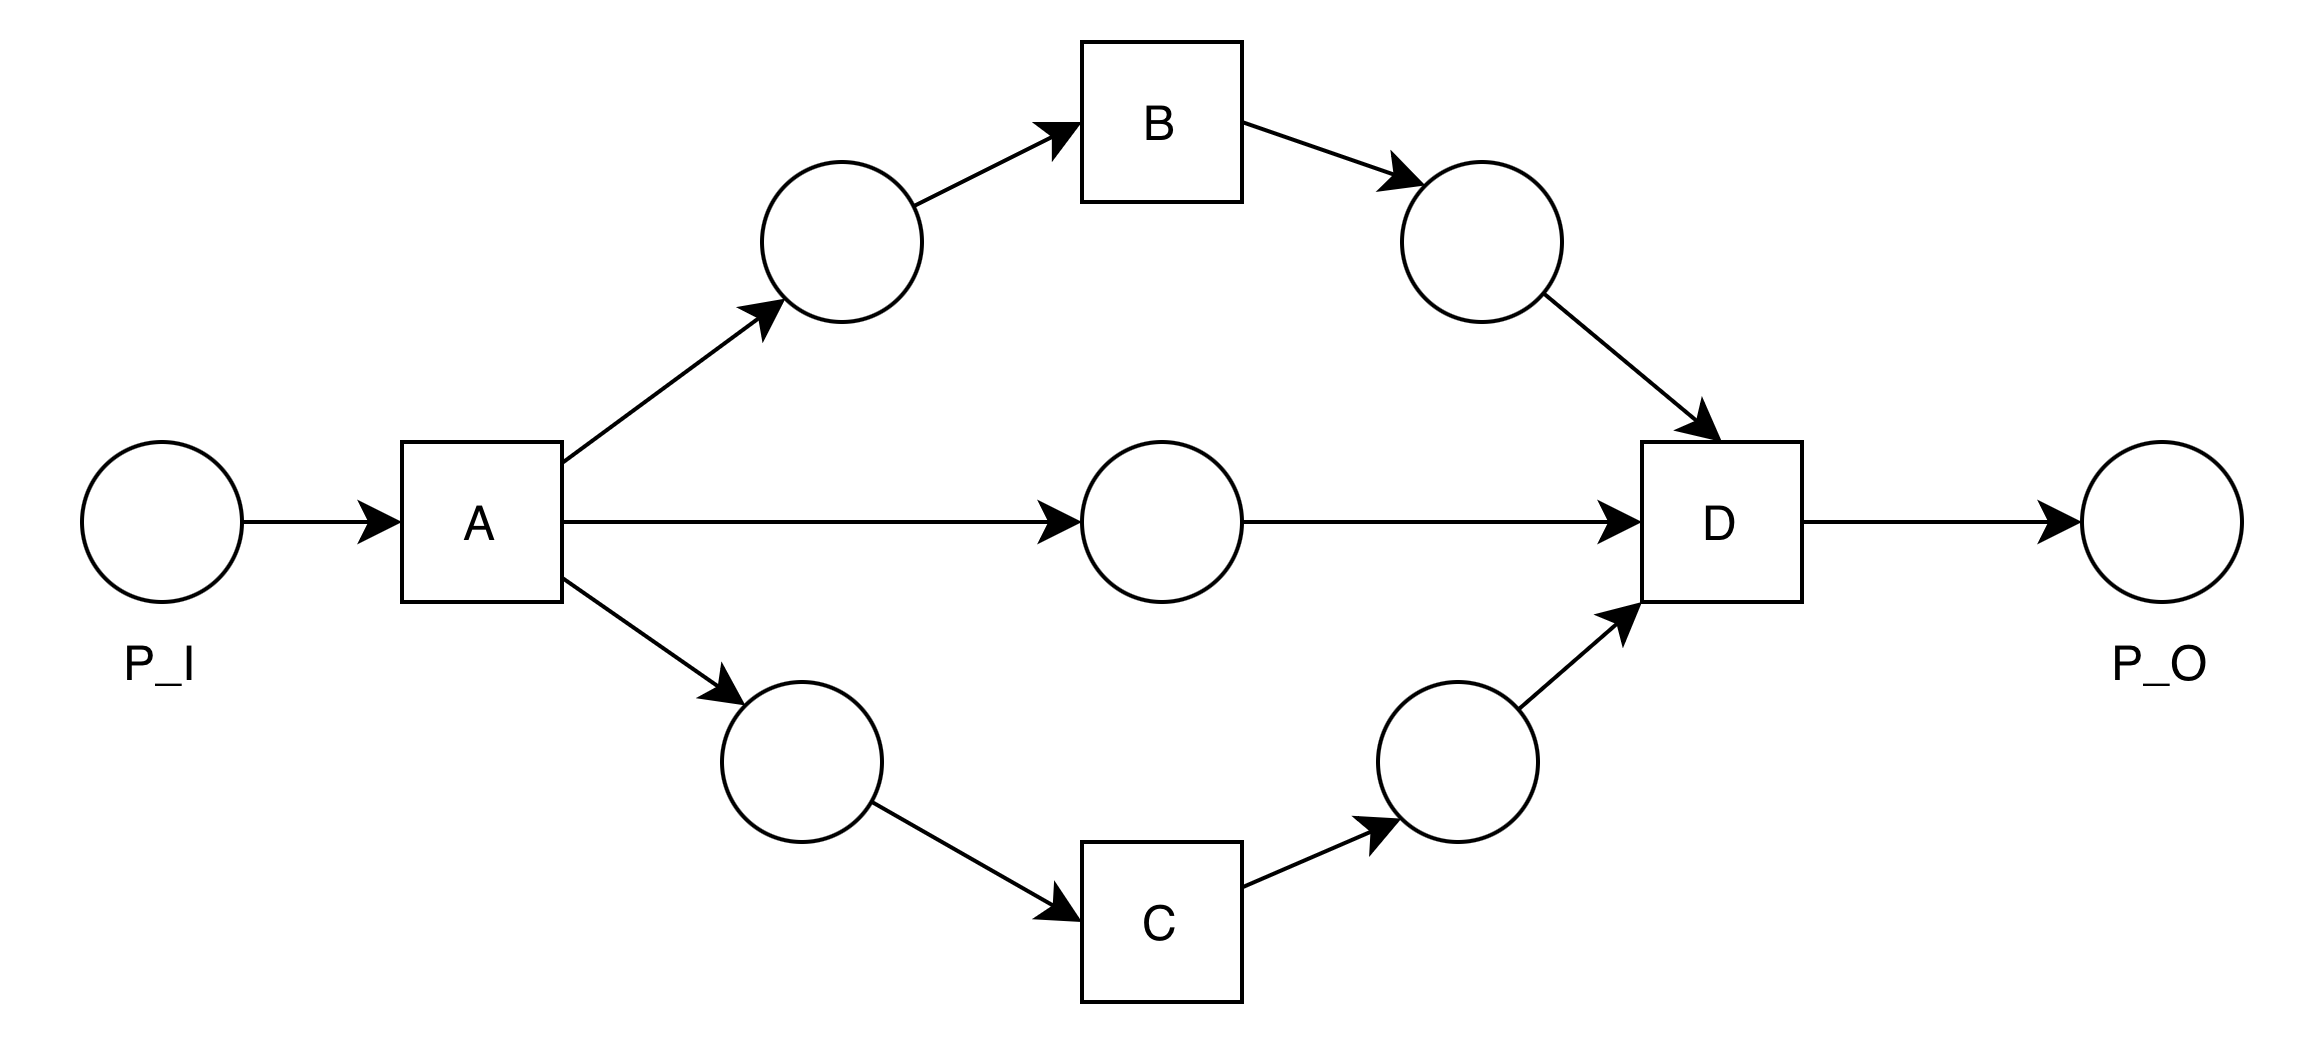
\includegraphics[width=0.7\textwidth]{../images/exercises/proc_discovery/alpha_miner-4.png}
        \caption{Petri Net Discovered using the Alpha Miner}
    \end{figure}
\end{itemize}


\subsection{Heuristic Miner}
\begin{exercise}{1}
Given the following event log:
\[L = [\langle a,e \rangle^5, \langle a,b,c,e \rangle^{10}, \langle a,c,b,e \rangle^{10}, \langle a,b,e \rangle^{1}, \langle a,c,e \rangle^{1},\]
\[
\langle a,d,e \rangle^{10}, \langle a,d,d,e \rangle^{2}, \langle a,d,d,d,e \rangle^{1}]
\]
use the Heuristic Miner algorithm to discover a process model from the event log, with a threshold of 0.7.
\end{exercise}
\paragraph{Solution:}
\begin{enumerate}
    \item First, we need to compute the frequency matrix:
    \begin{table}[H]
    \centering
    \begin{tabular}{c|cccccccc}
        & A & B & C & D & E \\
        \hline
        A & 0 & 11 & 11 & 13 & 5 \\
        B & 0 & 0 & 10 & 0 & 11 \\
        C & 0 & 10 & 0 & 0 & 11 \\
        D & 0 & 0 & 0 & 4 & 13 \\
        E & 0 & 0 & 0 & 0 & 0 \\
    \end{tabular}
    \caption{Frequency Matrix for the Event Log \(L\)}
    \end{table}
    Each cell \((x,y)\) contains the number of times activity \(x\) is directly followed by activity \(y\) in the event log.
    \item Next, we compute the dependency matrix, by applying the dependency measure formula to each pair of activities.
    Remember that the dependency measure is defined as:
    \[
    \begin{cases}
        \frac{|x\rightarrow y| - |y\rightarrow x|}{|x\rightarrow y| + |y\rightarrow x| + 1} & \text{if } x \neq y \\
        \frac{|x\rightarrow x|}{|x\rightarrow x| + 1} & \text{otherwise}
    \end{cases}
    \]
    Note that:
    \begin{itemize}
        \item Along the diagonal, we apply the second case of the formula;
        \item We can compute the upper triangle of the matrix, the lower triangle can be derived from it by simply swapping signs.
    \end{itemize}
    \begin{table}[H]
    \centering
    \begin{tabular}{c|cccccccc}
        & A & B & C & D & E \\
        \hline
        A & 0 & $\frac{11}{12}$ & $\frac{11}{12}$ & $\frac{13}{14}$ & $\frac{5}{6}$ \\
        B &  & 0 & $\frac{10 - 10}{21}$ & 0 & $\frac{11}{12}$ \\
        C &  &  & 0 & 0 & $\frac{11}{12}$ \\
        D &  &  &  & $\frac{4}{5}$ & $\frac{13}{14}$ \\
        E &  &  &  &  & 0 \\
    \end{tabular}
    \caption{Dependency Matrix for the Event Log \(L\)}
    \end{table}
    \item We can then build the dependency graph, using the given threshold.
    We create a node for each activity in the log, and add the directed edges for each pair of activities whose dependency measure is above the threshold:
    \begin{figure}[H]
        \centering
        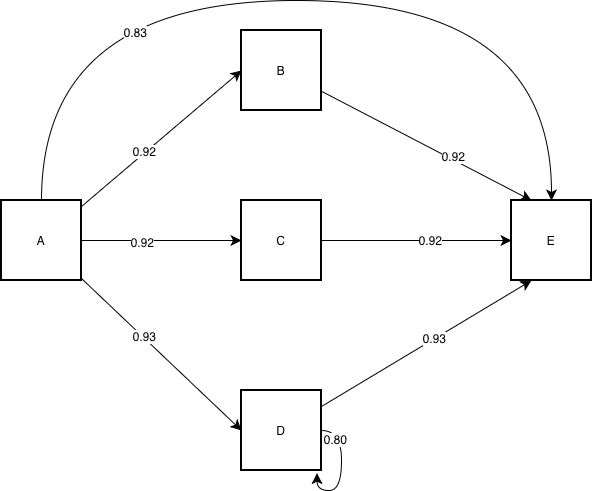
\includegraphics[width=0.7\textwidth]{../images/exercises/proc_discovery/heuristic_miner_1.png}
        \caption{Dependency Graph for the Event Log \(L\)}
    \end{figure}
\end{enumerate}

\begin{exercise}{2}
Given the following event log:
\[L_2 = \left[ \langle a,b,d,e \rangle^{80}, \langle a,d,b,e \rangle^{30}, \langle a,e \rangle^{2}, \langle a,b,c,d,e \rangle^{10} \right] \]
use the Heuristic Miner algorithm to discover the dependency matrix from the event log and build the dependency graph with a threshold of 0.9.
\end{exercise}
\paragraph{Solution:}
\begin{enumerate}
    \item First, we compute the frequency matrix:
    \begin{table}[H]
        \centering
        \begin{tabular}{c|ccccc}
            & A & B & C & D & E \\
            \hline
            A & 0 & 90 & 0 & 30 & 2 \\
            B & 0 & 0 & 10 & 80 & 30 \\
            C & 0 & 0 & 0 & 10 & 0 \\
            D & 0 & 30 & 0 & 0 & 90 \\
            E & 0 & 0 & 0 & 0 & 0 \\
        \end{tabular}
        \caption{Frequency Matrix for the Event Log \(L_2\)}
    \end{table}
    \item Next, we compute the dependency measure matrix:
    \begin{table}[H]
        \centering
        \begin{tabular}{c|ccccc}
            & A & B & C & D & E \\
            \hline
            A & 0 & $\frac{90}{91}$ & 0 & $\frac{30}{31}$ & $\frac{2}{3}$ \\
            B &  & 0 & $\frac{10}{11}$ & $\frac{50}{111}$ & $\frac{30}{31}$ \\
            C &  &  & 0 & $\frac{10}{11}$ & 0 \\
            D &  &  &  & 0 & $\frac{90}{91}$ \\
            E &  &  &  &  & 0 \\
        \end{tabular}
        \caption{Dependency measure Matrix for the Event Log \(L_2\)}   
    \end{table}
    \item Finally, we can build the dependency graph, using the given threshold.
    The resulting graph is the following:
    \begin{figure}[H]
        \centering
        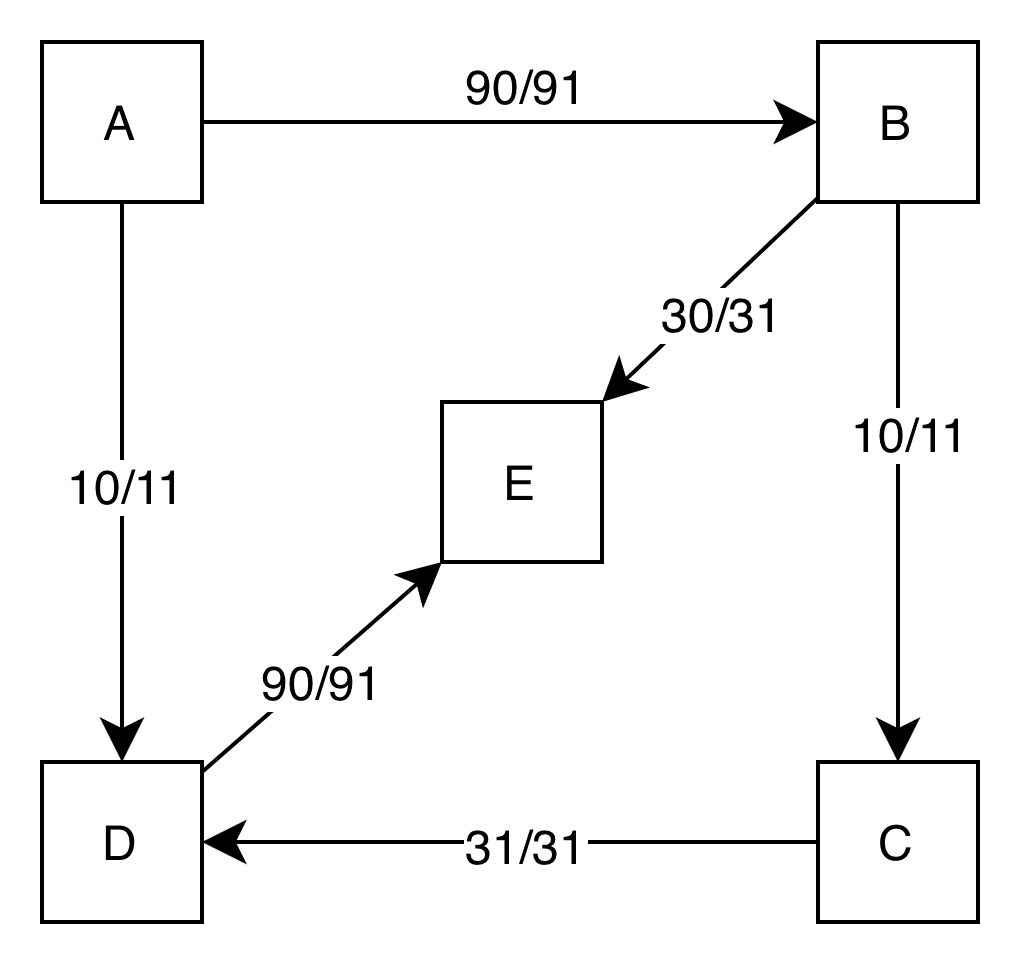
\includegraphics[width=0.37\textwidth]{../images/exercises/proc_discovery/heuristic_miner-2.png}
        \caption{Dependency Graph for the Event Log \(L_2\)}
    \end{figure}
\end{enumerate}

\begin{exercise}{3}
Given the following event log:
\[L_3 = \left[ \langle a,b,d \rangle^{100}, \langle a,c,b,d \rangle^{80}, \langle a,b,c,d \rangle^{2}, \langle a,c,d \rangle^{40}, \langle a,d \rangle^{1} \right] \]
Compute:
\begin{itemize}
    \item The frequency matrix;
    \item The dependency matrix;
    \item The dependency graph with a threshold of 0.9 and a threshold for direct succession of 1.
\end{itemize}
\end{exercise}
\paragraph{Solution:}
\begin{enumerate}
    \item First, we compute the frequency matrix:
    \begin{table}[H]
        \centering
        \begin{tabular}{c|cccc}
            & A & B & C & D \\
            \hline
            A & 0 & 102 & 120 & 1 \\
            B & 0 & 0 & 2 & 180 \\
            C & 0 & 80 & 0 & 42 \\
            D & 0 & 0 & 0 & 0 \\
        \end{tabular}
        \caption{Frequency Matrix for the Event Log \(L_3\)}
    \end{table}
    \item Next, we compute the dependency measure matrix:
    \begin{table}[H]
        \centering
        \begin{tabular}{c|cccc}
            & A & B & C & D \\
            \hline
            A & 0 & $\frac{102}{103}$ & $\frac{120}{121}$ & $\frac{1}{2}$ \\
            B & - & 0 & $\frac{-78}{83}$ & $\frac{180}{181}$ \\
            C & - & - & 0 & $\frac{42}{43}$ \\
            D & - & - & - & 0 \\
        \end{tabular}
        \caption{Dependency measure Matrix for the Event Log \(L_3\)}
    \end{table}
    The lower triangle can be derived from the upper triangle by swapping signs.
    \item Finally, we can build the dependency graph, using the given thresholds.
    The resulting graph is the following:
    \begin{figure}[H]
        \centering
        \includegraphics[width=0.4\textwidth]{../images/exercises/proc_discovery/Heuristic_Miner-3.png}
        \caption{Dependency Graph for the Event Log \(L_3\)}
    \end{figure}
\end{enumerate}

\subsection{Region Based Miner}

\begin{exercise}{1}
Construct a transition system applying the \textit{past with multiset abstraction} for the given log:
\[L = [\langle a,c,b,d \rangle, \langle a,b,c,d \rangle, \langle b,a,c,d \rangle]\]
\end{exercise}
\paragraph{Solution:}
\begin{enumerate}
    \item We create a starting state \(q_0\) with an empty multiset;
    \item We replay each trace in the log, updating the multiset and creating new states as needed. For instance, considering the first trace \(\langle a,c,b,d \rangle\):
    \begin{itemize}
        \item For the event \(a\), we add a transition from \(q_0\) to a new state \(q_1\) with multiset \(\{a\}\);
        \item For the event \(c\), we add a transition from \(q_1\) to \(q_2\) with multiset \(\{a,c\}\);
        \item For the event \(b\), we add a transition from \(q_2\) to \(q_3\) with multiset \(\{a,b,c\}\);
        \item \dots
    \end{itemize}
    Continuing this process for all traces, we obtain the following transition system:
    \begin{figure}[H]
        \centering
        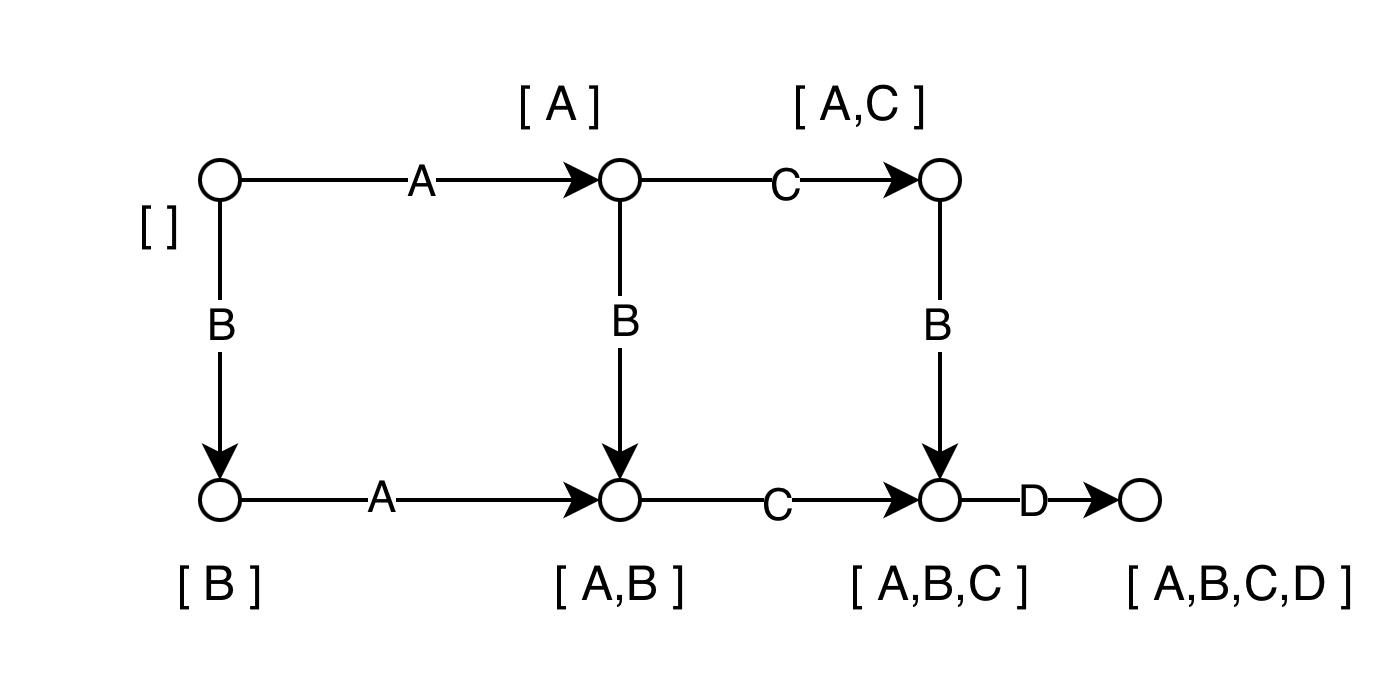
\includegraphics[width=0.7\textwidth]{../images/exercises/proc_discovery/region_miner-1.png}
        \caption{Transition System using Past with Multiset Abstraction}
    \end{figure}
\end{enumerate}

\begin{exercise}{2}
Given the previous transition system, compute the resulting Petri net.
\end{exercise}
\paragraph{Solution:}
\begin{enumerate}
    \item We identify the minimal, non-trivial regions in the transition system. In this case, we have:
    \begin{figure}[H]
        \centering
        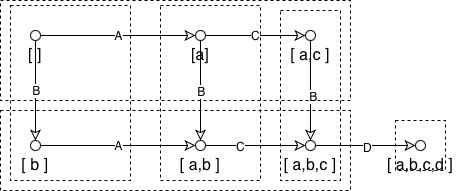
\includegraphics[width=0.7\textwidth]{../images/exercises/proc_discovery/region_miner-2_1.png}
        \caption{Identified Regions from the Transition System}
    \end{figure}
    \item We then create a place for each region. 
    All the transition entering a region will have an arc to the corresponding place, and all transitions leaving the region will have an arc from the place.
    This results in the following Petri net:
    \begin{figure}[H]
        \centering
        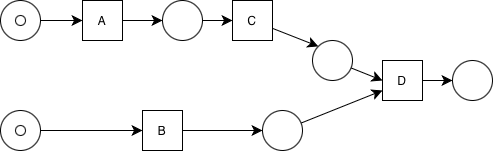
\includegraphics[width=0.7\textwidth]{../images/exercises/proc_discovery/region_miner-2_2.png}
        \caption{Petri Net Derived from the Transition System}
    \end{figure}
\end{enumerate}

\begin{exercise}{3}
Given the following event log:
\[L = [\langle a,b,c,d \rangle^3, \langle a,c,b,d \rangle^2, \langle a,e,d \rangle^1]\] 
build the process model using the Region Based Miner algorithm with \textit{past with set abstraction}.
\end{exercise}
\paragraph{Solution:}
\begin{enumerate}
    \item First, we create the transition system using past with set abstraction:
    \begin{figure}[H]
        \centering
        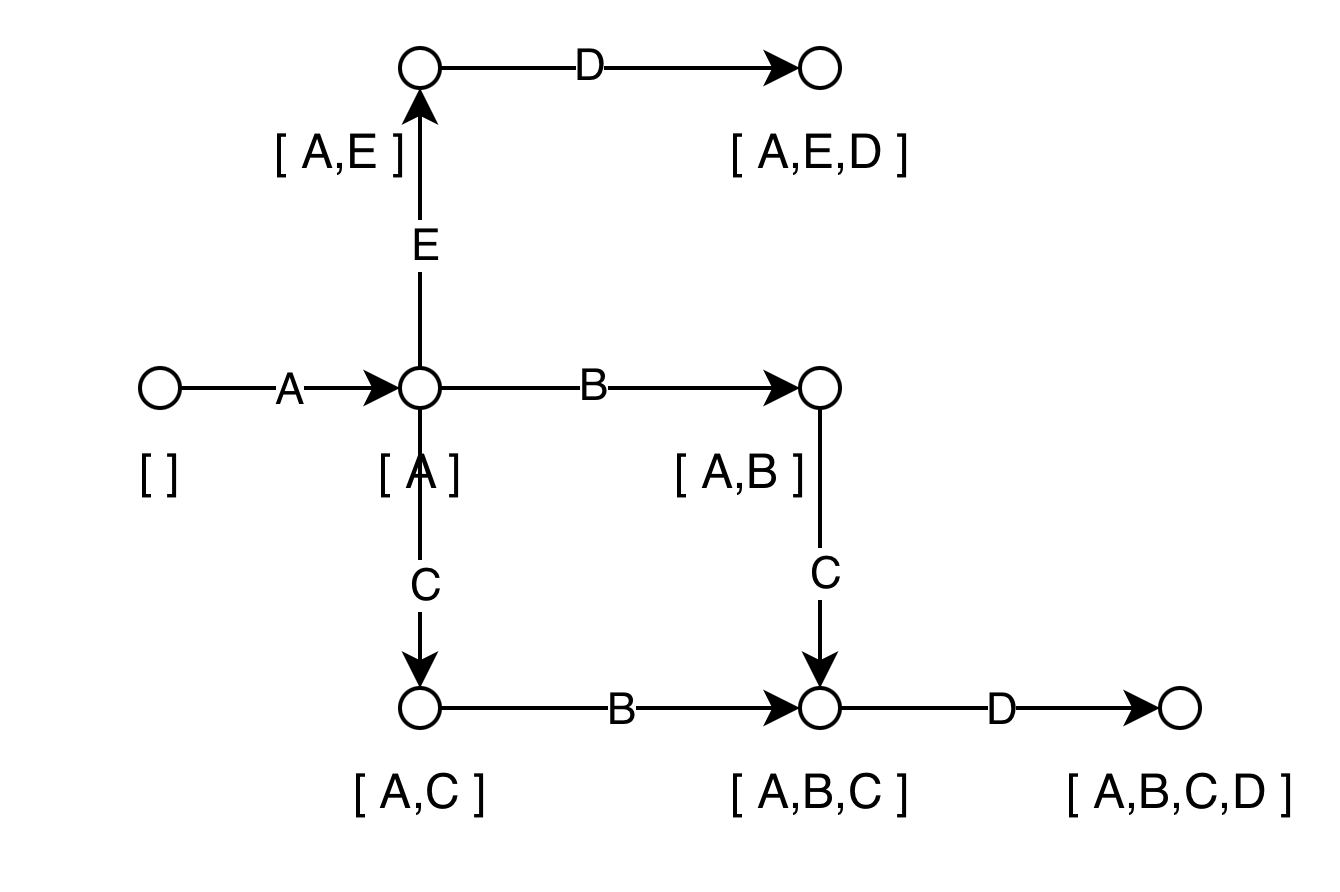
\includegraphics[width=0.4\textwidth]{../images/exercises/proc_discovery/region_miner-3_1.png}
        \caption{Transition System using Past with Set Abstraction}
    \end{figure}
    \item Next, we identify the minimal, non-trivial regions in the transition system:
    \begin{figure}
        \centering
        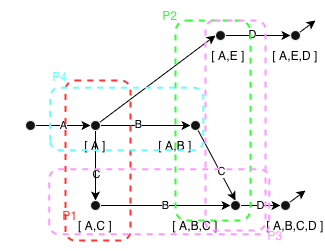
\includegraphics[width=0.6\textwidth]{../images/exercises/proc_discovery/region_miner-3_2.png}
        \caption{Identified Regions from the Transition System}
    \end{figure}
    We have the following regions:
    \begin{itemize}
        \item \textbf{P1}: $A$ enters, $B,E$ leaves;
        \item \textbf{P2}: $B,E$ enter, $D$ leaves;
        \item \textbf{P3}: $C,E$ enter, $D$ leaves;
        \item \textbf{P4}: $A$ enters, $C,E$ leaves.
    \end{itemize}
    \item Finally, we create a place for each region and connect them to the transitions according to the entering and leaving activities.
    We also add the input and output places. The resulting Petri net is the following:
    \begin{figure}[H]
        \centering
        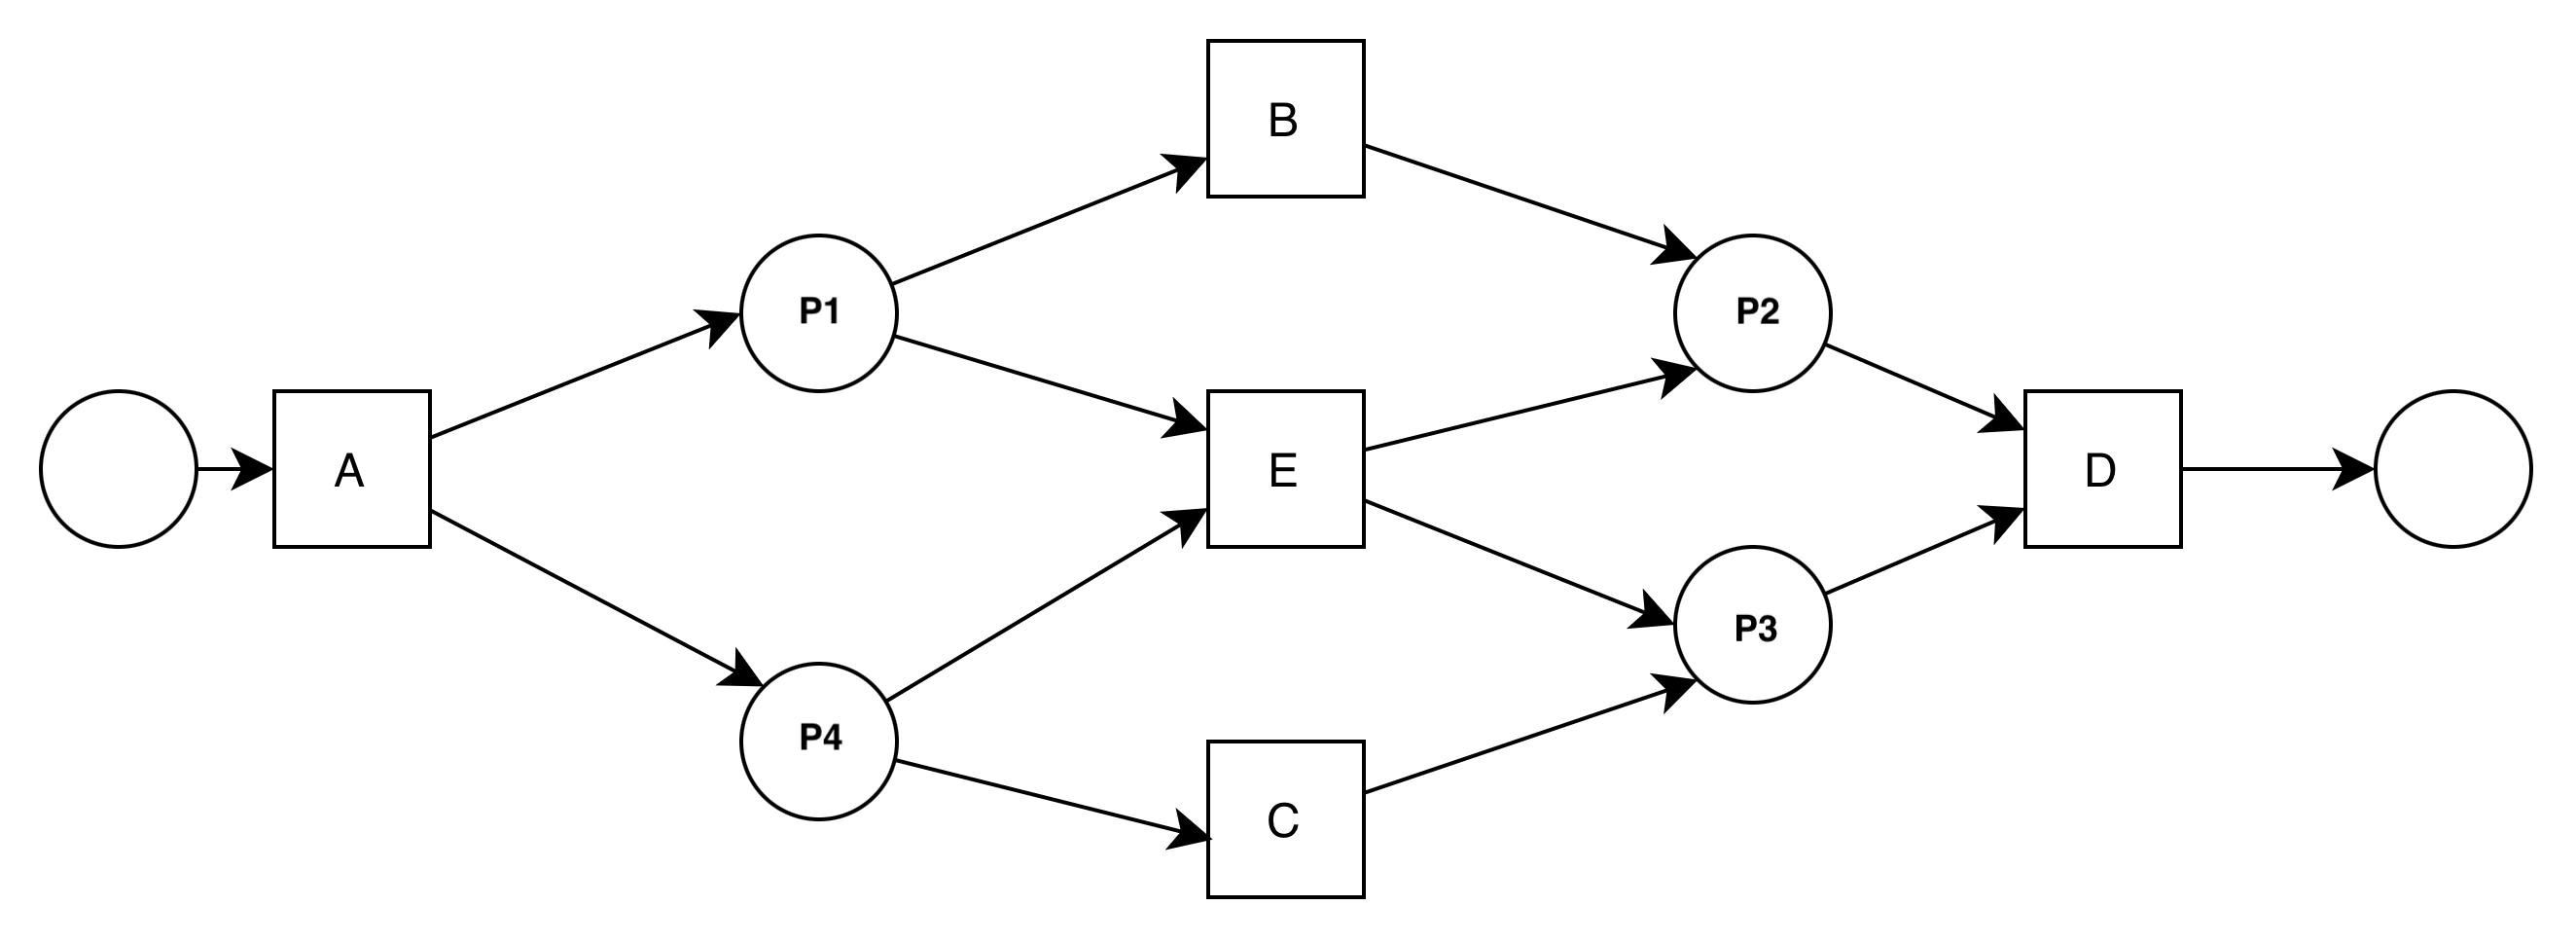
\includegraphics[width=0.7\textwidth]{../images/exercises/proc_discovery/region_miner-3_3.png}
        \caption{Petri Net Discovered using the Region Based Miner}
    \end{figure}
\end{enumerate}

\begin{exercise}{4}
Given the following event log:
\[L = [\langle a,b,d \rangle^{100}, \langle a,c,b,d \rangle^{80}, \langle a,b,c,d \rangle^{2}, \langle a,c,d \rangle^{40}, \langle a,d \rangle^{1}]\]
Use the Region Based Miner algorithm with \textit{past with set abstraction} to discover a Petri Net.
\end{exercise}
\paragraph{Solution:}
\begin{enumerate}
    \item We first create the transition system using past with set abstraction:
    \begin{figure}[H]
        \centering
        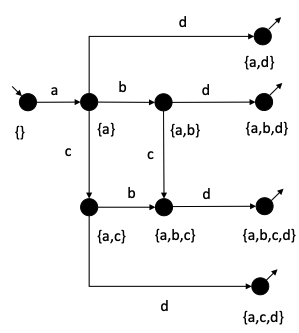
\includegraphics[width=0.7\textwidth]{../images/exercises/proc_discovery/region_miner-4_1.png}
        \caption{Transition System using Past with Set Abstraction}
    \end{figure}
    \item Next, we identify the minimal, non-trivial regions in the transition system:
    \begin{itemize}
        \item First, we can easily identify the easier regions, corresponding to places \(p_i\) and \(p_o\):
        \begin{itemize}
            \item $P_I$: \(A\) leaves, nothing enters;
            \item $P_O$: \(D\) enters, nothing leaves.
        \end{itemize}
        \item Then, we can identify the other regions, remembering that all equally labeled transitions must behave the same way, 
        with respect to the region:
        \begin{itemize}
            \item $P_1$: \(B\) enters, nothing leaves;
            \item $P_2$: \(C\) enters, nothing leaves;
            \item $P_3$: \(A\) enters, \(D\) exits;
            \item $P_4$: \(A\) enters, \(B\) exits. Note that for this region, we have to get a little creative.
            Since the simplest region that can come to mind is not valid as the top and bottom \(D\) transition enter, while the two middle \(D\) transitions leave.
            We can however create a region where \(A\) enters, and \(B\) exit by going around the \(D\) transitions, including in the region the two
            terminal nodes at the top and bottom.
            \item $P_5$: \(A\) enters, \(C\) exits. Similarly, also for this region we have to include the two nodes in the top half of the transition system.
        \end{itemize}
    \end{itemize}
    \item Finally, we create a place for each region and connect them to the transitions according to the entering and leaving activities.
    \begin{figure}[H]
        \centering
        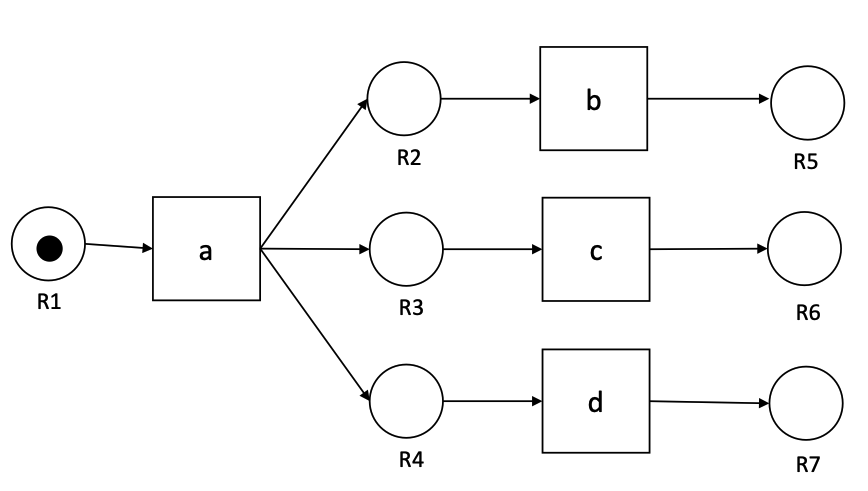
\includegraphics[width=0.6\textwidth]{../images/exercises/proc_discovery/region_miner-4_2.png}
        \caption{Petri Net Discovered using the Region Based Miner}
    \end{figure}
\end{enumerate}

\subsection{Inductive Miner}
\begin{exercise}{1}
Given the following event log:
\[L = [\langle a,b,c,d \rangle^3,
    \langle a,c,b,d \rangle^4,
    \langle a,b,c,e,f,b,c,d \rangle^2,
    \langle a,c,b,e,f,b,c,d \rangle^2,\]
\[
    \langle a,b,c,e,f,c,b,d \rangle,
    \langle a,c,b,e,f,b,c,e,f,c,b,d \rangle 
\]
use the Inductive Miner algorithm to discover a process model from the event log.
\end{exercise}
\paragraph{Solution:}
\begin{enumerate}
    \item To begin, we first need to build the directly-follows graph (DFG) from the event log.
    We create a node for each activity in the log, and add directed edges between nodes that directly follow each other in any trace.
    For example if activity \(a\) is directly followed by activity \(b\) in some trace, we add a directed edge from node \(a\) to node \(b\).
    The resulting DFG is the following:
    \begin{figure}[H]
        \centering
        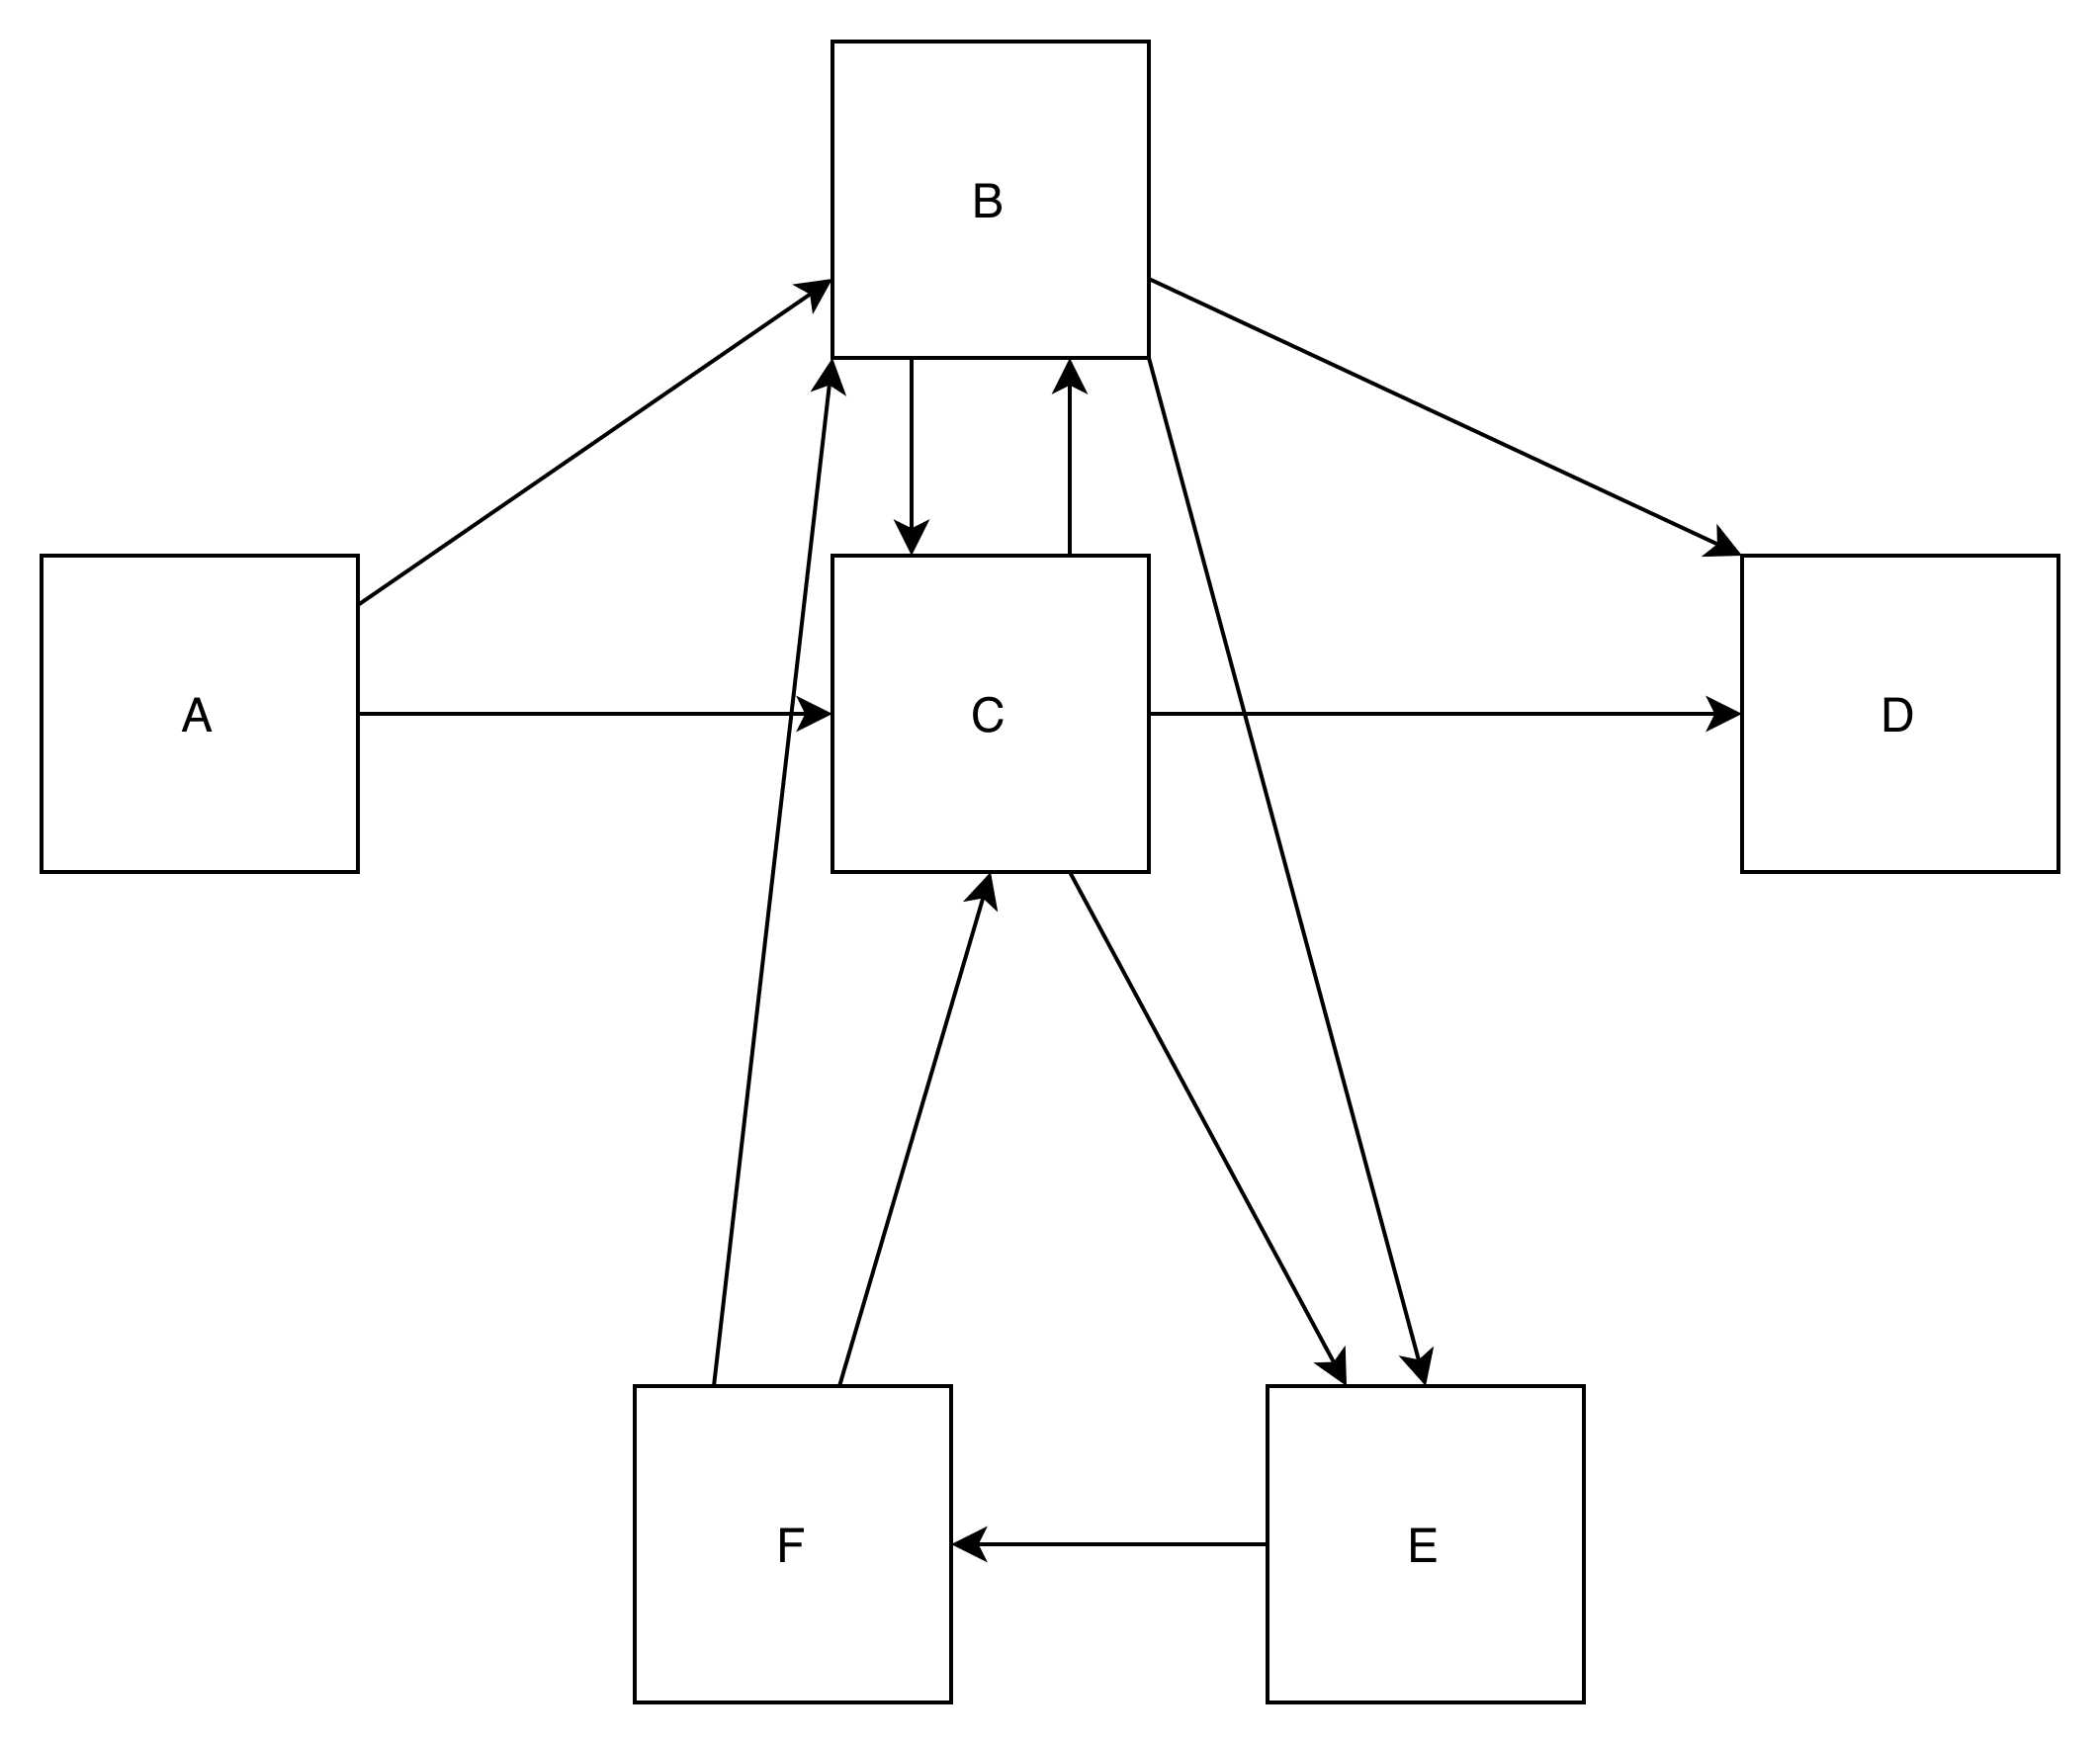
\includegraphics[width=0.5\textwidth]{../images/exercises/proc_discovery/inductive_miner-1_1.png}
        \caption{Directly-Follows Graph for the Event Log \(L\)}
    \end{figure}
    \item Next, we analyze the DFG to identify the possible splits:
    \begin{itemize}
        \item An exclusive cut is clealy not prossible;
        \item Two sequence cuts are possible: one between \(a\) and the rest of the activities, and another between \(d\) and the rest of the activities;
        We end up with terminal nodes \(a\) and \(d\).
    \end{itemize}
    \item We can now analyze the subgraphs between the identified sequence cuts:
    \begin{figure}[H]
        \centering
        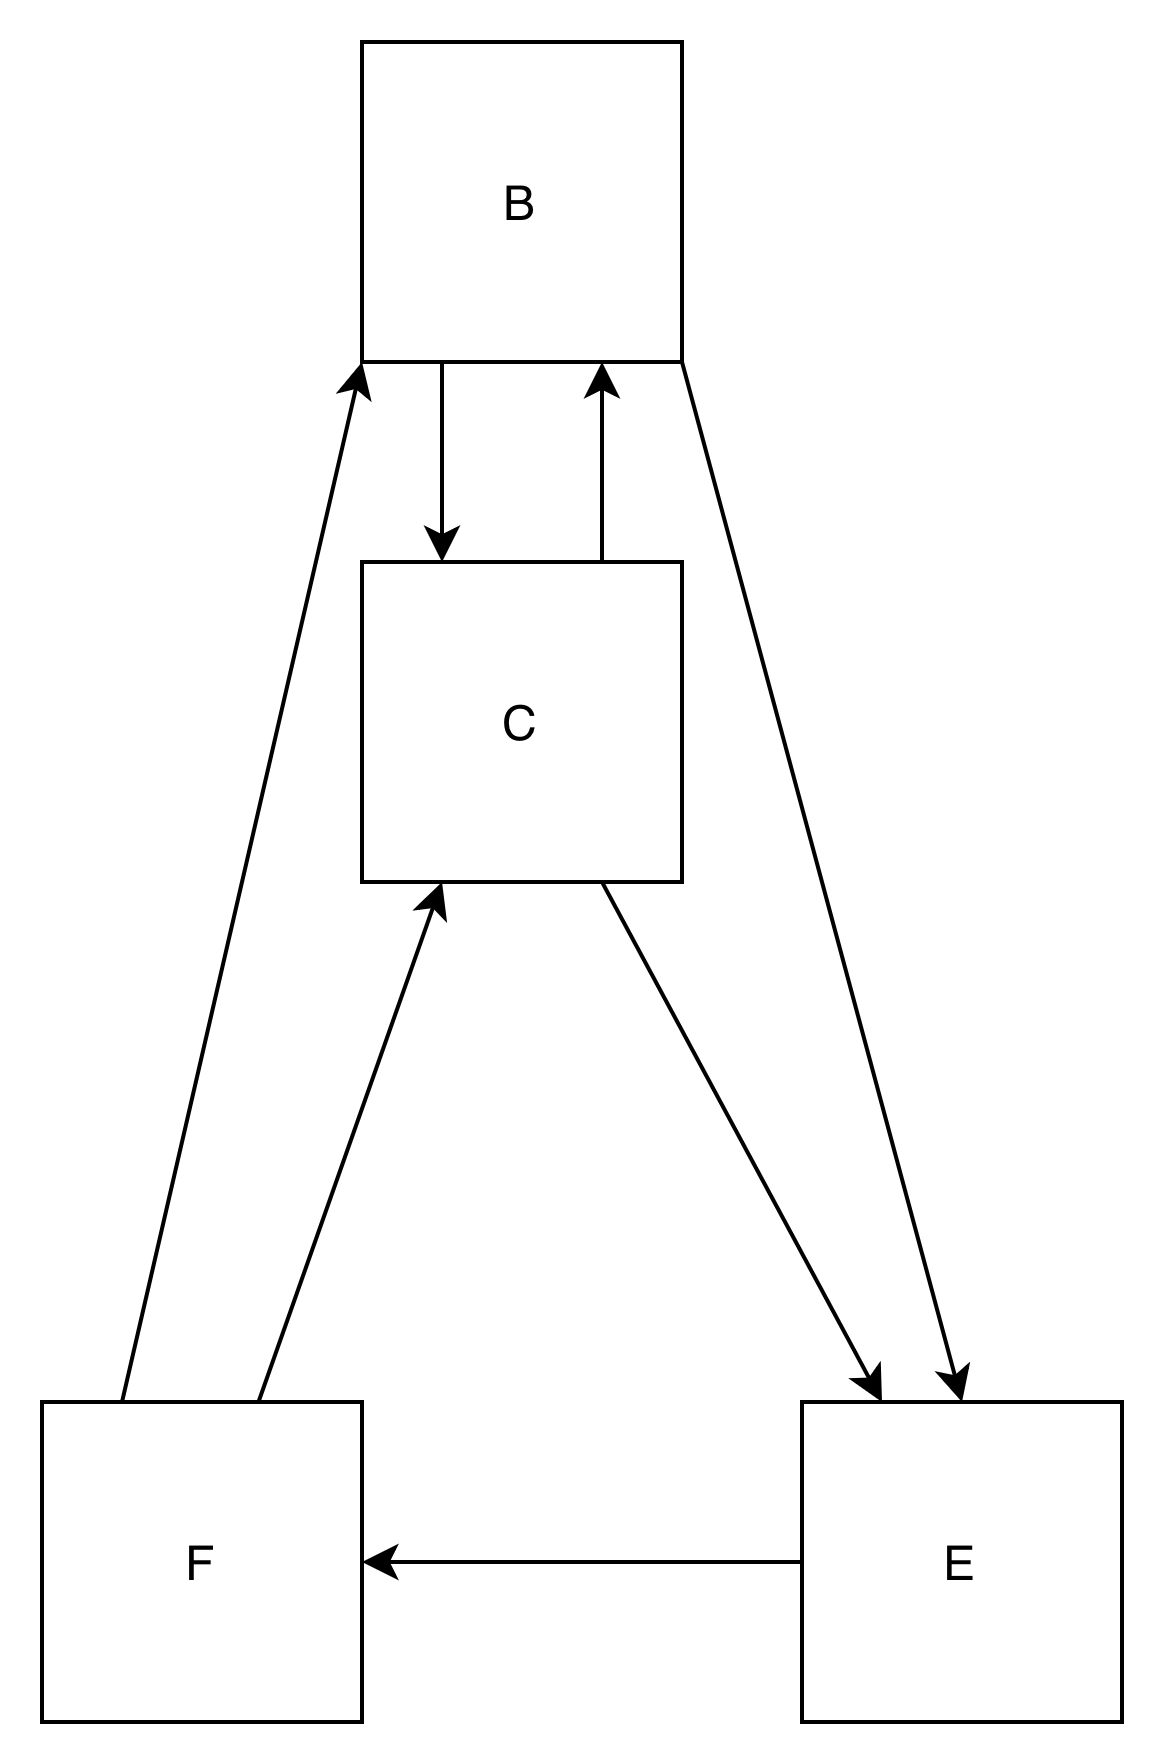
\includegraphics[width=0.25\textwidth]{../images/exercises/proc_discovery/inductive_miner-1_2.png}
        \caption{Subgraph between the Sequence Cuts}
    \end{figure}
    and the respectives traces:
    \[L = [\langle b,c \rangle^3,
    \langle c,b \rangle^4,
    \langle b,c,e,f,b,c \rangle^2,
    \langle c,b,e,f,b,c \rangle^2,\]
    \[
    \langle b,c,e,f,c,b \rangle,
    \langle c,b,e,f,b,c,e,f,c,b \rangle 
    \]
    Analyzing the log, we can see that is probable to have a redo loop between \(b,c\) and \(e,f\).
    Also, all the other cuts are not possible. We can therefore apply a parallel cut, obtaining two subgraphs:
    \begin{figure}[H]
        \centering
        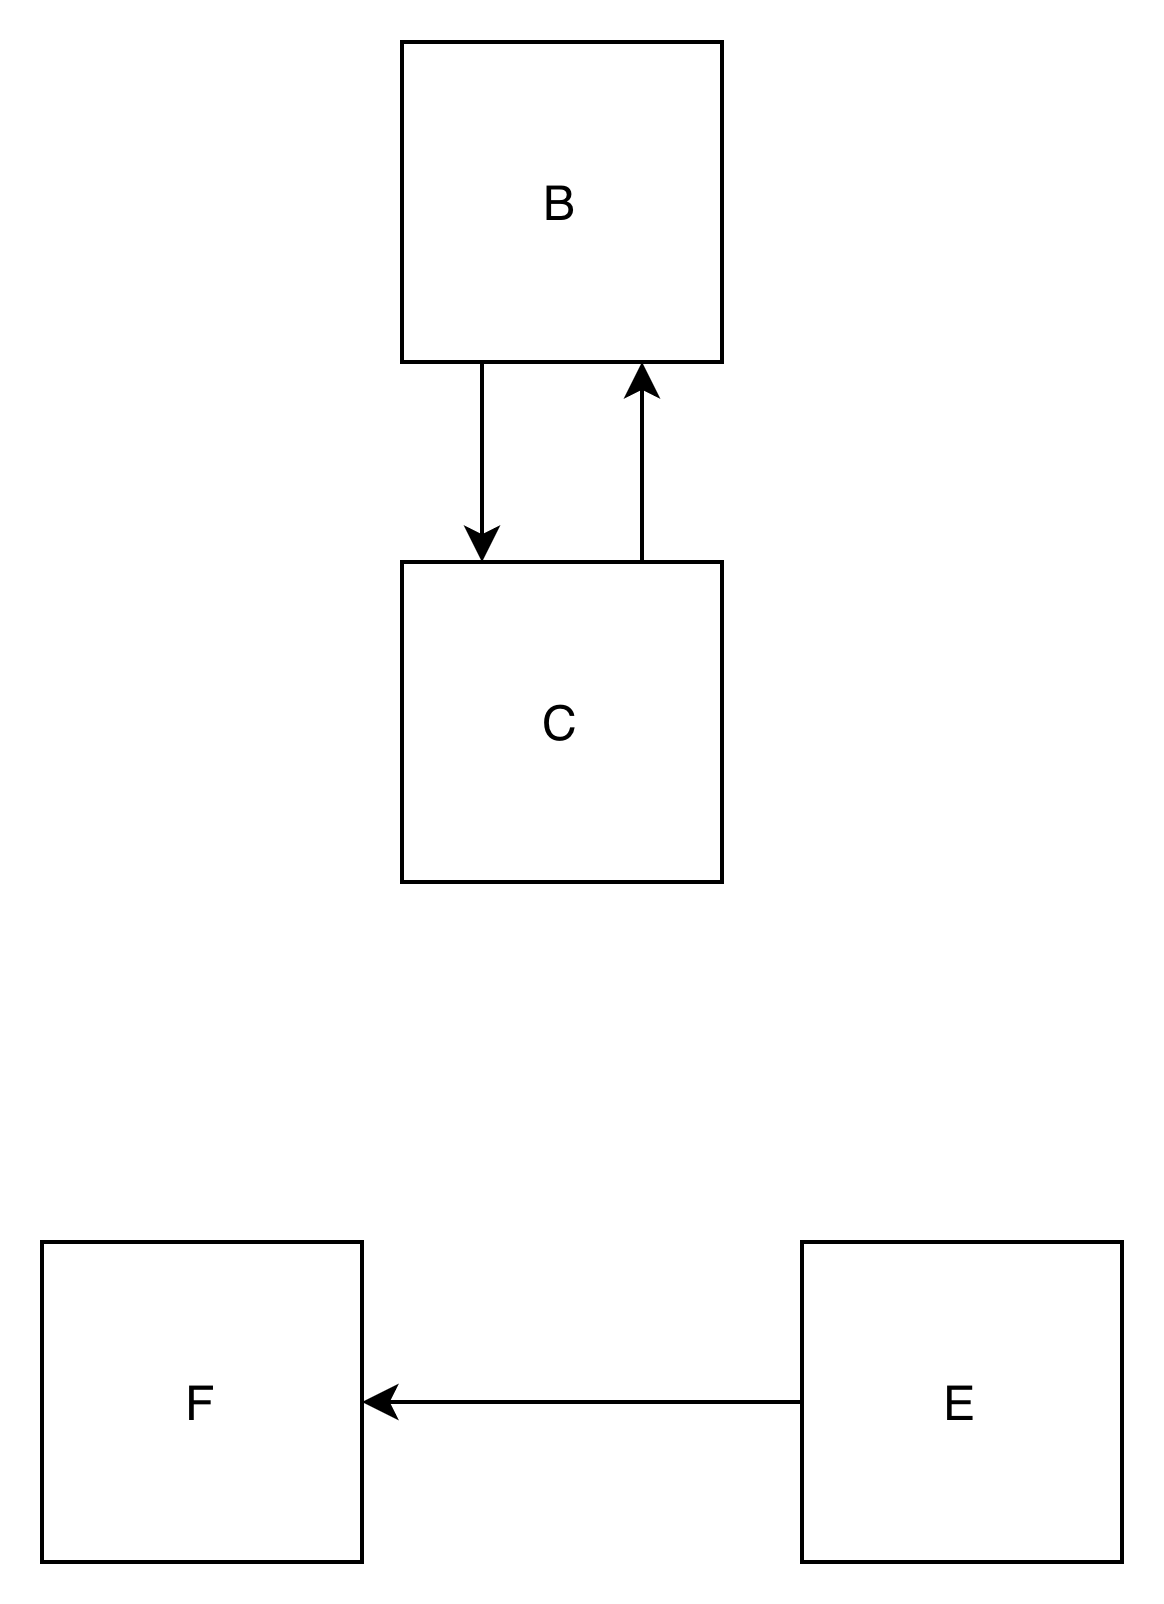
\includegraphics[width=0.25\textwidth]{../images/exercises/proc_discovery/inductive_miner-1_3.png}
        \caption{Subgraphs after Applying the Parallel Cut}
    \end{figure}
    \item Finally, we can analyze each of the subgraphs:
    \begin{itemize}
        \item The first subgraph contains activity \(b\) and \(c\), interconnected.
        This means we can do a parallel cut, obtaining two terminal nodes \(b\) and \(c\);
        \item The second subgraph contains activity \(e\) and \(f\), connected in sequence.
        We can apply a sequence cut, obtaining two terminal nodes \(e\) and \(f\).
    \end{itemize}
    \item We can now construct the process model by combining all the identified cuts and terminal nodes:
    \begin{figure}[H]
        \centering
        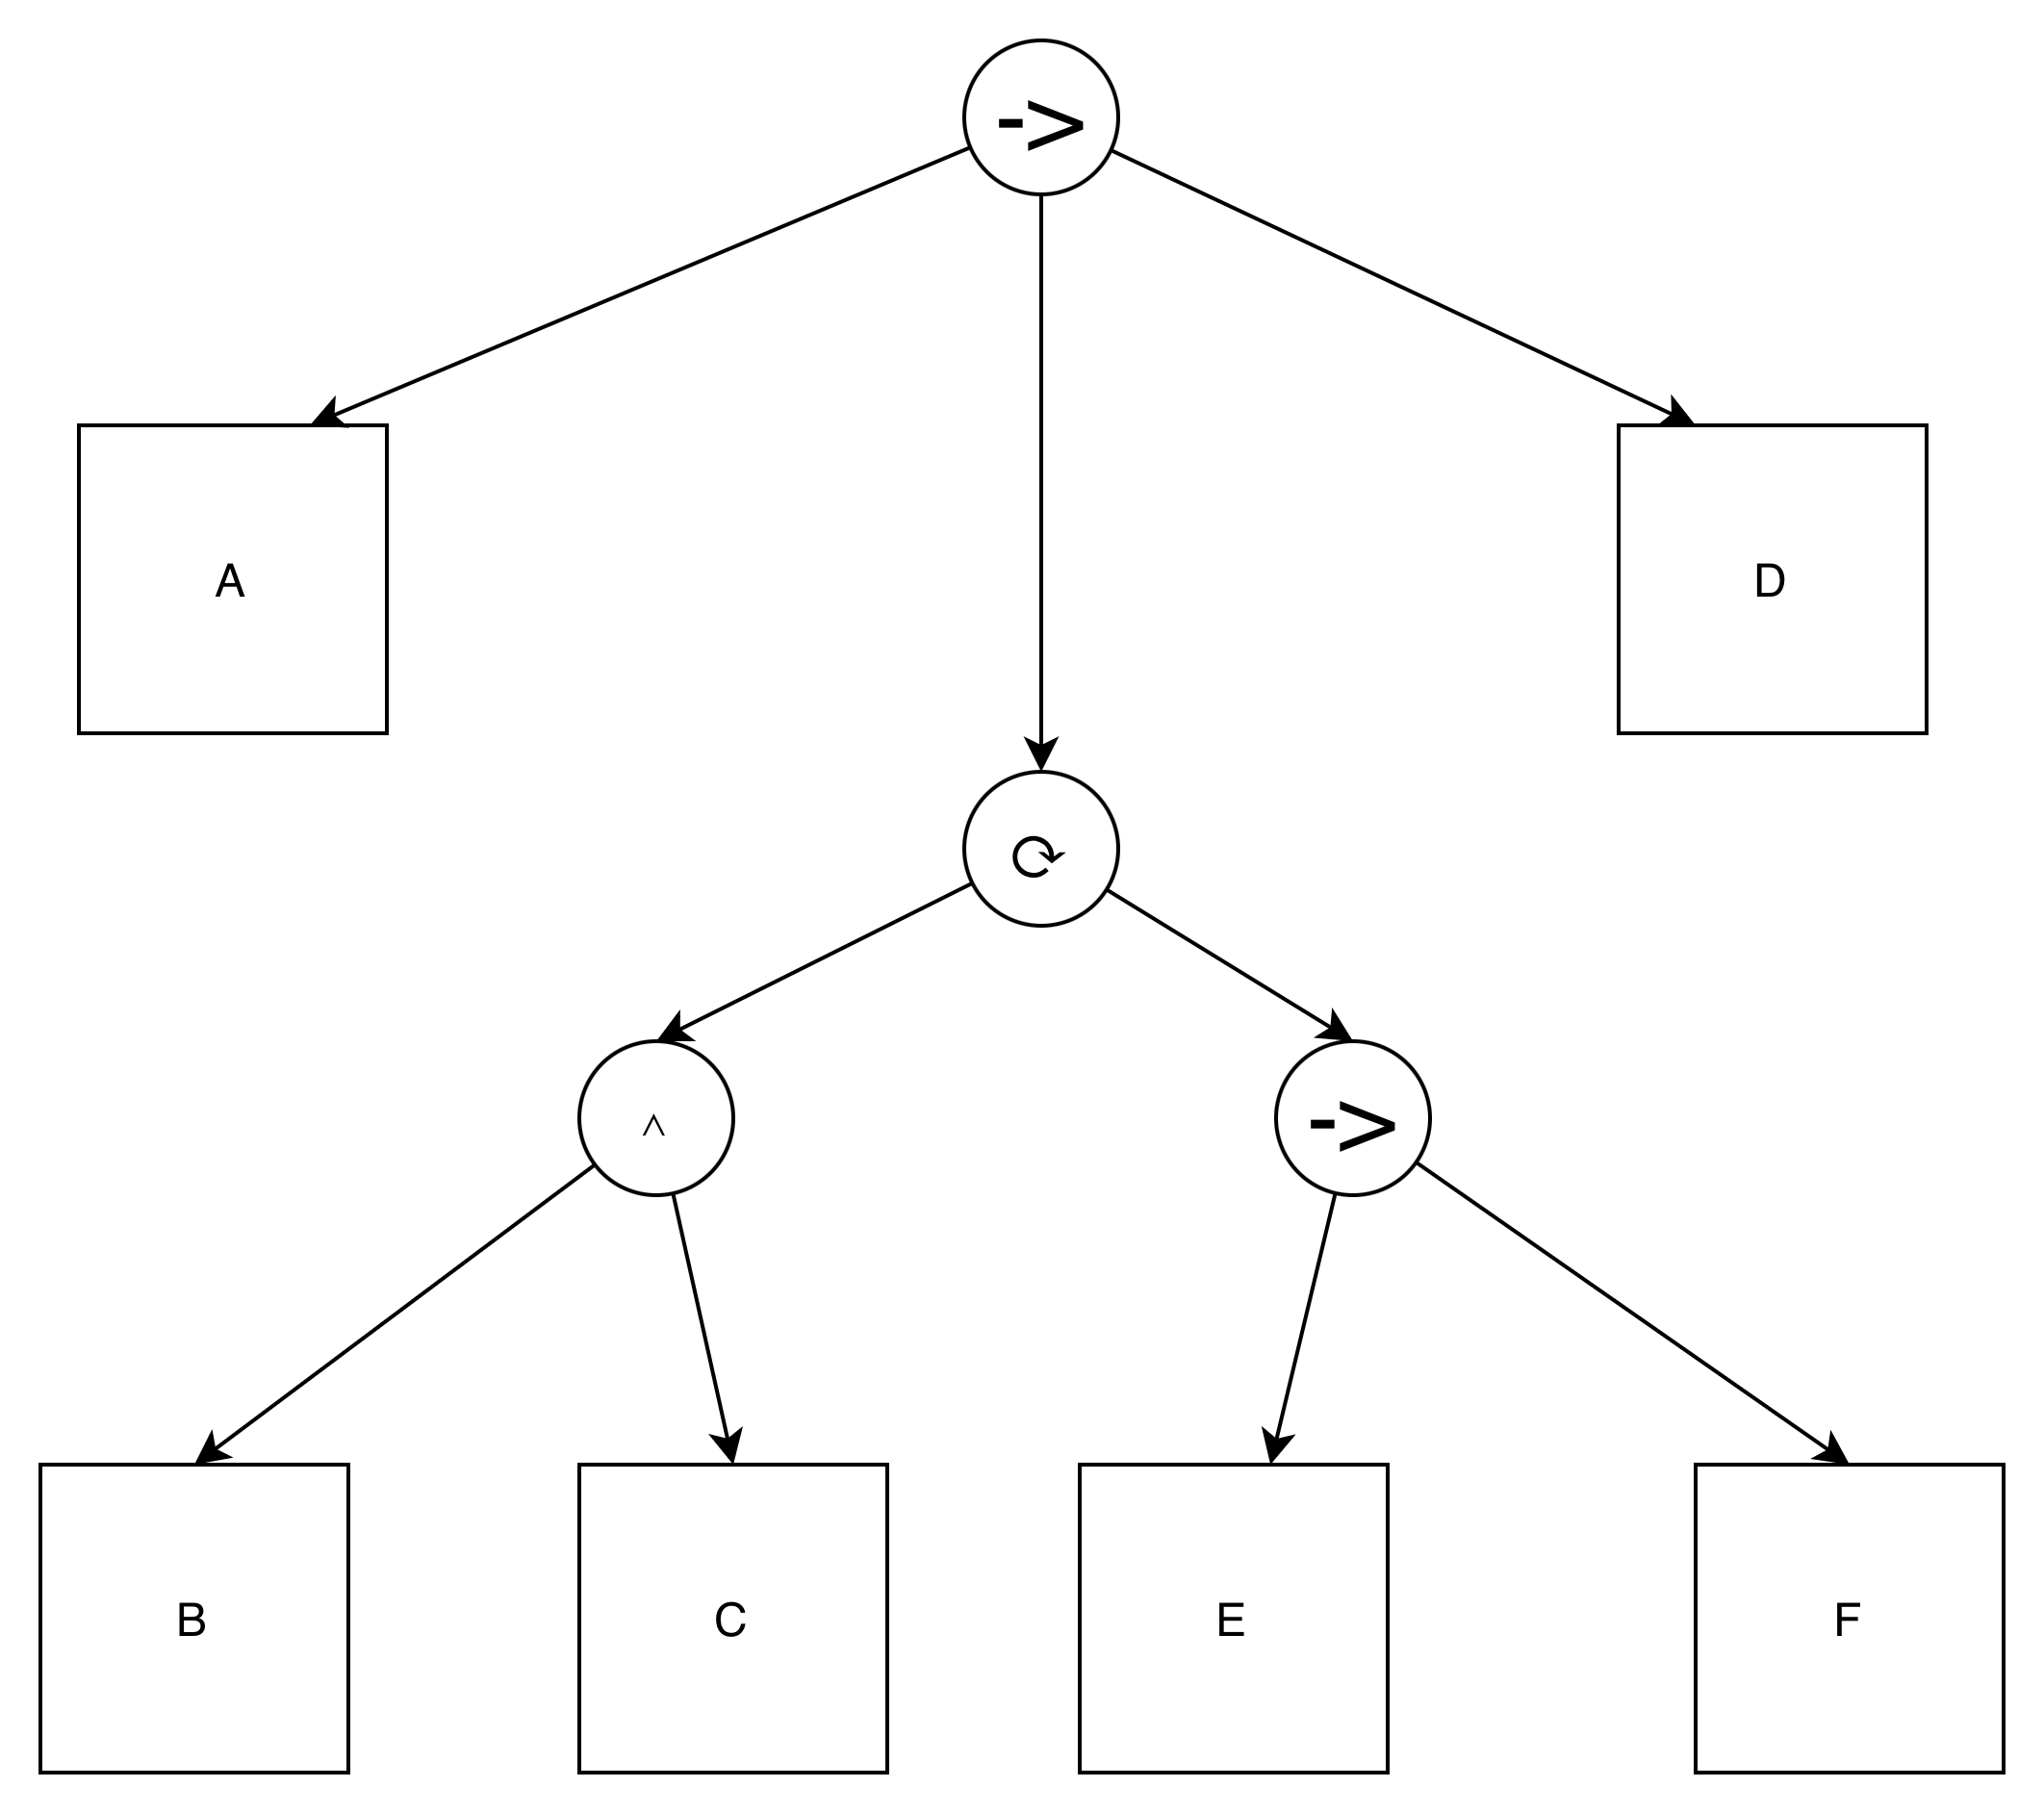
\includegraphics[width=0.4\textwidth]{../images/exercises/proc_discovery/inductive_miner-1_4.png}
        \caption{Process Model Discovered using the Inductive Miner}
    \end{figure}
\end{enumerate}

\begin{exercise}{2}
Given the following event log:
\[L = [\langle a,c,d \rangle^{45}, \langle b,c,d \rangle^{42}, \langle a,c,e \rangle^{38}, \langle b,c,e \rangle^{22}]\]
use the Inductive Miner algorithm to discover a process model from the event log.
\end{exercise}
\begin{comment}
    #TODO: add solution
\end{comment}

\begin{exercise}{3}
Given the following event log:
\[L = [\langle a,b,d \rangle^{100}, \langle a,c,b,d \rangle^{80}, \langle a,b,c,d \rangle^{2}, \langle a,c,d \rangle^{40}, \langle a,d \rangle^{1}]\]
use the Inductive Miner algorithm to discover a process model from the event log.
\end{exercise}
\begin{comment}
    #TODO: add solution
\end{comment}